\section{Imperfect plate and spheres}
\label{sec:3:imperfect-plates}

In reality, the shield and/or the sphere do not offer a completely smooth surface and thus the separation altering the Casimir interaction marginally.
Even thermal vibrations can induce small imperfections on the plate.
To quantify and estimate the change in the Casimir force, a selection of different and relevant imperfections with amplitude $\Delta \mathscr{L}$ shown in \cref{fig:3:imperfect-plates} have been studied with numerical methods.
\begin{figure}[!htbp]
  \centering
  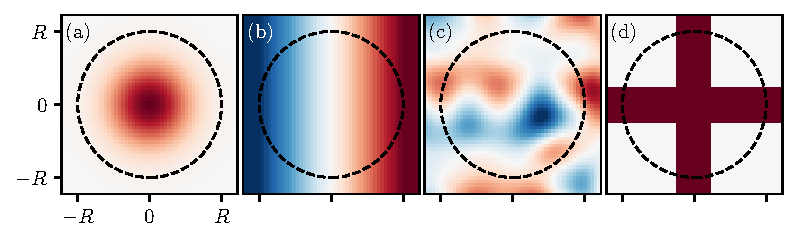
\includegraphics[width=\textwidth]{../figures/casimir/imperfect-plates-advanced.pdf}
  \caption{A selection of imperfect plates. \textbf{(a)} A simple gaussian deformation in the same size as the sphere. \textbf{(b)} Linearly inclining plate or a tilted flat plate. \textbf{(c)} Uneven and noisy but uniformly random surface realized using \textit{Perlin noise} \cite{Perlin_1985}. \textbf{(d)} A cross-shape in the center of the plate.}
  \label{fig:3:imperfect-plates}
\end{figure}
\begin{enumerate}
  \item[\textbf{(a)}] A \textit{gaussian deformation} of the plate can be used to describe a range of possible imperfections in the size of the sphere. Thermal excitations of the shield, as discussed in \cref{cha:the-shield} look very similar for a shield in the size of the sphere in front of it. Because of the importance of this kind of imperfections, a positive and negative displacement in the form of a gaussian distribution is considered.
  \item[\textbf{(b)}] For the description of large (i.e. locally linearizable) irregularities in the shield, \textit{linear deflections} or a constant tilting of the plate are also relevant. For small a tilting the resulting change in casimir interactions should be neglectable and no change compared to a parallel plate is expected.
  \item[\textbf{(c)}] Similar arguments hold for the consideration of a random uniformly distributed displacement noise qualitatively given by \textit{Perlin noise} function \cite{Perlin_1985}. This type of noise is commonly used in computer science and produces a uniform smooth pseudo-random noise that is often used to imitate surface roughness \cite{Perlin_1985}. Equidistant grid-points are defined, each of which is assigned with a pseudo-random gradient. The noise function follows this gradient in the vicinity of a grid-point and interpolation methods generate smooth transitions. Due to the uniformness, no large deviations from an ideal parallel plate is expected.
  \item[\textbf{(d)}] A structure in the shield, like e.g. a \textit{centered cross} might improve stability and rigidity of the shield. Thermal vibrations could be reduced by such a design but the effect and amplification of the Casimir interaction has to be investigated.
\end{enumerate}
The resulting Casimir potentials numerically calculated in the proximity force approximation (PFA) for each of the discussed imperfect surfaces with amplitude $\Delta \mathscr{L}$ is shown in \cref{fig:3:casimir-imperfect-plates}.
\begin{figure}[!htbp]
  \centering
  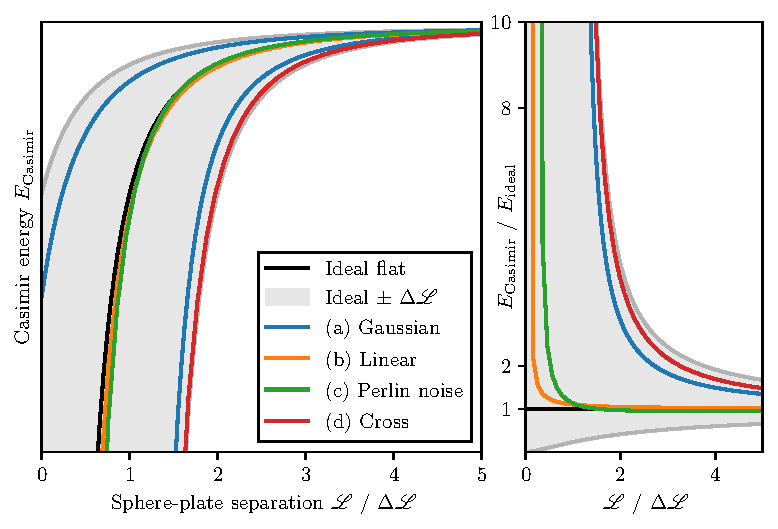
\includegraphics[width=\textwidth]{../figures/casimir/casimir-potential-imperfect-plates-relative.pdf}
  \caption{Casimir energy for the different imperfect plates in \cref{fig:3:imperfect-plates}. The dashed-blue line represents a negative gaussian displacement reducing the overall Casimir force. The shaded region is given by an ideal plate separated by a distance of $\mathscr{L} \pm \Delta\mathscr{L}$ from the sphere. It becomes evident, that for large separations, the local imperfections are neglectable.}
  \label{fig:3:casimir-imperfect-plates}
\end{figure}
As logically expected, all variations are upper bounded by moving the ideal flat plate closer (or farther) to the sphere by a distance $\Delta \mathscr{L}$. Interestingly it seems like that for the gaussian distribution the overestimation is not particularly large.
A evenly tilted plate as well as a uniformly rough plate don't change the Casimir interactions noticeably even at small separations.
If the plate and sphere are far separated ($\mathscr{L} \gg R$) these local imperfections are neglectable as the relative effect of them decreases and becomes less noticeable.
But especially for small shields in the size of the particles and close separations the considerations from this section are important.